%%%%%%%%%%%%%%%%%%%%%%%%%%%%%%%%%%%%%%%%%%%%%%%%%%%%
% This will help you in writing your homebook
% Remember that the character % is a comment in latex
%
% chapter 1
\chapter{Reference model development}
\label{chap1}

%%%%%%%%%%%%%%%%%%%%%%%%%%%%%%%%%%%%%%%%%%%%%%%%%%%%%%%%%%%
% you can organize a chapter using sections -> \section{Simulating an inverter}
% or subsections -> \subsection{simulating a particular type of inverter}

%%%%%%   First section

According to our group number our goal is to design a FIR filter with a parallelism of 8 and a parallelism of 11.

\section{Full Adder}

Adders are one of the most used digital components in computer processors. In general an adder is a digital circuit that implements the sum of two numbers expressed on N bits.\\
In particular, a full adder (FA) is characterized by three inputs and two outputs. If we consider a one-bit full adder, the three inputs are the two numbers to sum and the input carry. The outputs are the sum and the output carry. A schematic diagram of a one-bit full adder is shown in figure \ref{fig:fa}-A. % here is the reference to the figure below

% Below is shown how you can insert a figure. If you give a label to the figure, you can refer to the figure using \ref{figure_label} as shown above. 

	\begin{figure}[ht]
	\centering
	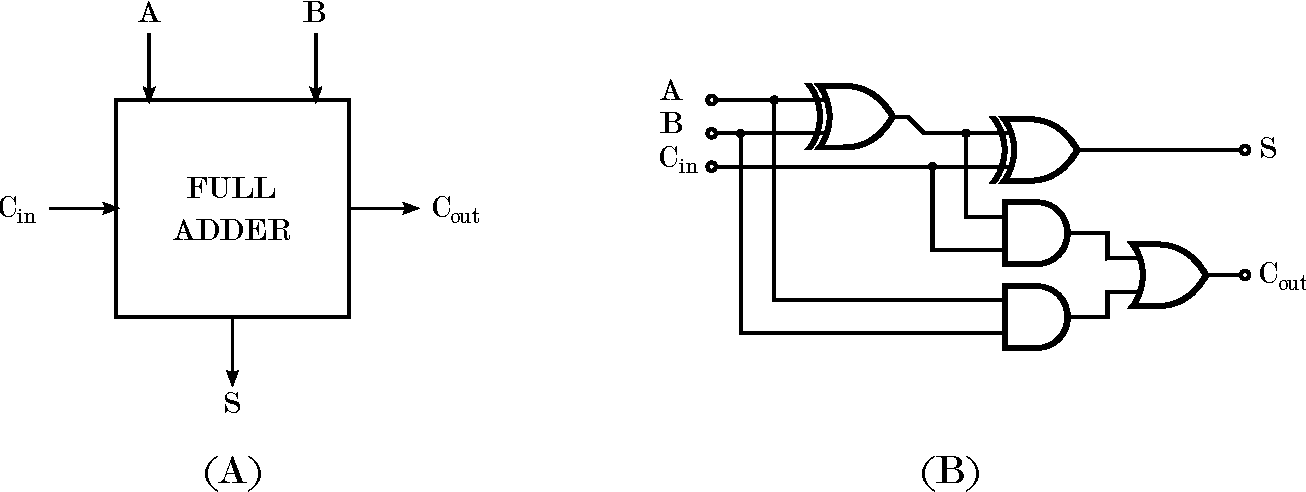
\includegraphics[width=\textwidth]{chapters/figures/fa} 
	\caption{(A) Schematic symbol of a 1-bit full adder. A and B are the operands, Cin is the carry-in while Cout and S are the carry-out and the sum, respectively. (B) Logic diagram of the 1-bit full adder.}
	\label{fig:fa}  % here is the figure label
	\end{figure}

The truth table of the one-bit full adder is shown in table \ref{tab:1}. % here is the reference to the table below

% Below is an example of how to create a simple table. You can create a reference (using \ref{table_label}) to tables too if you give them a label.

	\begin{table}[ht]
	\centering
	\begin{tabular}{ccc}
	\toprule
	A B Cin & S & Cout\\
	\midrule
	0 0 0 & 0 & 0\\
	1 0 0 & 1 & 0\\
	0 1 0 & 1 & 0\\
	1 1 0 & 0 & 1\\
	0 0 1 & 1 & 0\\
	1 0 1 & 0 & 1\\
	0 1 1 & 0 & 1\\
	1 1 1 & 1 & 1\\
	\bottomrule
	\end{tabular}
	\caption{Truth table of a 1-bit full adder.}
	\label{tab:1} % here is the table label
	\end{table}
	
From the truth table we can easily derive the logic equations that describe the full adder:

% Below is an example of how to write equations.

	\begin{equation}
	S = A \oplus B \oplus C_{in}
	\label{eq:1}
	\end{equation}

	\begin{equation}
	C_{out} = AB + C_{in}( A \oplus B)
	\label{eq:2}
	\end{equation}
	
\subsection{Area and power estimation}

A simple Bash script has been written to automatise the calculus of area and power starting from the layout of the circuit. The script takes in input the SVG (which is the primary Inkscape's format) description of the layout and it extracts all the necessary information. The output of the script is a .txt file containing different data.\\
The output text file of the full adder is reported below.

\verbatiminput{chapters/files/planar_FA_area_power.txt}  

% The command \verbatiminput allows you to import the text (e.g, some code or the output resulting from running a program or a script) written in a file.
% You can also include some text in this way:
%	\begin{verbatim}
%		text here
%	\end{verbatim}

% Below is shown how to create an itemize. An alternative to itemize is enumerate that allows you to generate a numbered list. It is used in the same way as itemize:
%	\begin{enumerate}
%		\item bla1
%		\item bla2
%		\item bla3
%	\end{enumerate}

To summarize, the planar full adder is characterized by:
\begin{itemize}
\item Delay = 3 clock cycles;
\item Area = $2.7\ \mu m^2$;
\item Power = $10.53\ \mu W$.
\end{itemize}
	
\section{Ripple Carry Adder}

A Ripple-carry adder (RCA) is a more complex adder composed by a cascade of more full adders. It is used to add N-bit numbers and its name derives from the fact that the carry propagates from a full adder to the next one.\\
\dots \dots \dots \\
\dots \dots \\
\dots